\newpage % Rozdziały zaczynamy od nowej strony.
\section{Warstwy}

\subsection{DENSE}

%http://zsi.tech.us.edu.pl/~nowak/si/SI_w4.pdf 

%https://www.fuw.edu.pl/~jarekz/SIECI/wyklad3.pdf 

Jest to najbardziej podstawowy typ warstwy, w której każdy neuron uzyskuje informacje ze wszystkich wejść. Następnie agreguje te dane, przy uwzględnieniu wag odpowiadającym wejściom i przy wykorzystaniu swojej funkcji aktywacji wylicza wartość wyjściową neuronu. 

Często jedna warstwa gęsto połączona nie wystarcza by poprawnie rozwiązywać dane zadanie klasyfikacji, dlatego wykorzystuje się kilka takich warstw ze sobą połączonych tak, że wyjścia jednej warstwy są jednocześnie wejściami kolejnej warstwy. Należy jednak pamiętać, że funkcja aktywacji musi być wtedy funkcją nieliniową. Obecnie najczęściej wykorzystywaną funkcją aktywacji jest funkcja ReLU opisana poniższym wzorem: 

%https://en.wikipedia.org/wiki/Activation_function
$$f(x) = max(0,x) = \left\{\begin{matrix}
         & 0,\ dla\ x \leq 0 \\
         & x,\ dla\ x > 0
    \end{matrix}\right.
$$

\subsection{Warstwa konwolucyjna}

% https://towardsdatascience.com/text-classification-rnns-or-cnn-s-98c86a0dd361
% https://towardsdatascience.com/a-comprehensive-guide-to-convolutional-neural-networks-the-eli5-way-3bd2b1164a53

% http://www.wildml.com/2015/11/understanding-convolutional-neural-networks-for-nlp/

Sieci używające warstw konwolucyjnych (takie sieci oznaczane są często jako CNN) z reguły wykorzystywane są w ramach analizy obrazu. Działają one w oparciu o różne filtry przemieszczające się systematycznie po macierzy obrazu. Dany obraz może być jednocześnie analizowany przez wiele filtrów przemieszczających się z różnym skokiem. Pozwala to na naukę rozpoznawania różnych cech obrazu umożliwiających zagadnienia klasyfikacji. Kolejne warstwy konwolucyjne można ze sobą łączyć pozwalając na rozpoznawanie coraz bardziej zaawansowanych cech obrazu.

W przypadku analizy tekstu macierzą wejściową dla warstwy konwolucyjnej jest macierz o wymiarze AxB, gdzie A to liczba słów w zdaniu, a B to rozmiar embeddingu. Natomiast, ze względu na strukturę danych, sama ekstrakcja cech dokonywana przez filtr może przebiegać tylko w ramach wymiaru A, gdyż dane wzdłuż wymiaru B reprezentują unikalne cechy danego słowa i nie powinny być agregowane.


\subsection{Pooling}

%https://www.quora.com/What-is-pooling-in-a-convolutional-neural-network 

%https://www.quora.com/What-is-max-pooling-in-convolutional-neural-networks 

Zadaniem warstwy poolingu jest zmniejszenie wymiarowości macierzy uzyskanej z poprzedniej warstwy (bardzo często występuję tuż po warstwie konwolucyjnej). Można ten proces porównać do przeprowadzania operacji zmniejszania rozdzielczości obrazu. Operacja ta polega na systematycznym przesuwaniu stałego okna po macierzy wejściowej i dokonywania pewnej formy agregacji danych (wybór elementu o najwyższej wartości, wyliczenie średniej z wartości elementów) na elementach macierzy zawierających się w bieżącym oknie. Dzięki takiemu zabiegowi kolejne warstwy sieci mogą skupiać się na analizie i wykrywaniu bardziej skomplikowanych wzorców w oparciu o cechy uwypuklone przez warstwę poolingu. 

 

Najbardziej popularną formą poolingu jest max pooling, który polega na wybieraniu elementu o najwyższej wartości spośród elementów w oknie. Na rysunku XXX przedstawiono przykład takiej operacji przy zastosowaniu okna o rozmiarze 2x2 i przesunięciu wynoszącym 2. 

\begin{figure}[!h]
    \label{fig:max_pooling}
    \centering 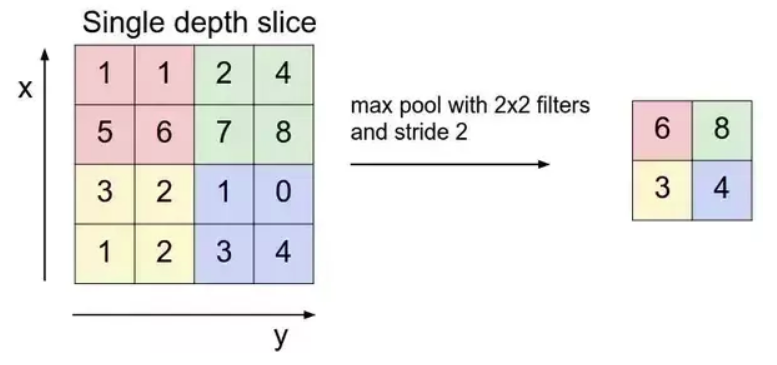
\includegraphics[width=0.75\linewidth]{max_pooling.png}
    \caption{Wynik operacji max poolingu}
\end{figure}


\subsection{RNN}

% http://colah.github.io/posts/2015-08-Understanding-LSTMs/ 

% https://towardsdatascience.com/illustrated-guide-to-recurrent-neural-networks-79e5eb8049c9 


Neuronowa sieć rekurencyjna (RNN) powstała z myślą o przewidywaniu kolejnych elementów sekwencji. Jako wejście przyjmuje kolejne elementy sekwencji, ale w przeciwieństwie do sieci typu feedforward posiada także swój wewnętrzny  stan, w ramach którego zawarta jest informacja o poprzednich wejściach. Sieć tego typu charakteryzuje się jednak bardzo istotną wadą, mianowicie boryka się ona z problem zanikającego gradientu. Jest on spowodowany naturą propagacji wstecznej i wiąże się z coraz mniejszym wpływem początkowych elementów sekwencji na wyjście modelu. Aby temu zaradzić zostały wprowadzone nowe architektury warstw, jedną z nich jest warstwa typu LSTM.

\subsection{LSTM}

% https://towardsdatascience.com/illustrated-guide-to-lstms-and-gru-s-a-step-by-step-explanation-44e9eb85bf21

Warstwa typu LSTM składa się nuronów zawierających w sobie wiele pośrednich operacji. Poniżej zostaną omówione najważniejsze z nich.

\begin{figure}[!h]
    \label{fig:lstm_diagram}
    \centering 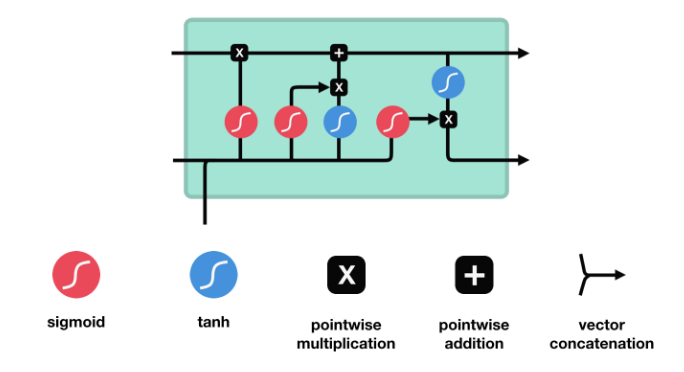
\includegraphics[width=1\linewidth]{lstm_diagram.png}
    \caption{Przepływ danych w jedynczym neuronie LSTM}
\end{figure}


\begin{figure}[!h]
    \label{fig:lstm_gates}
    \centering 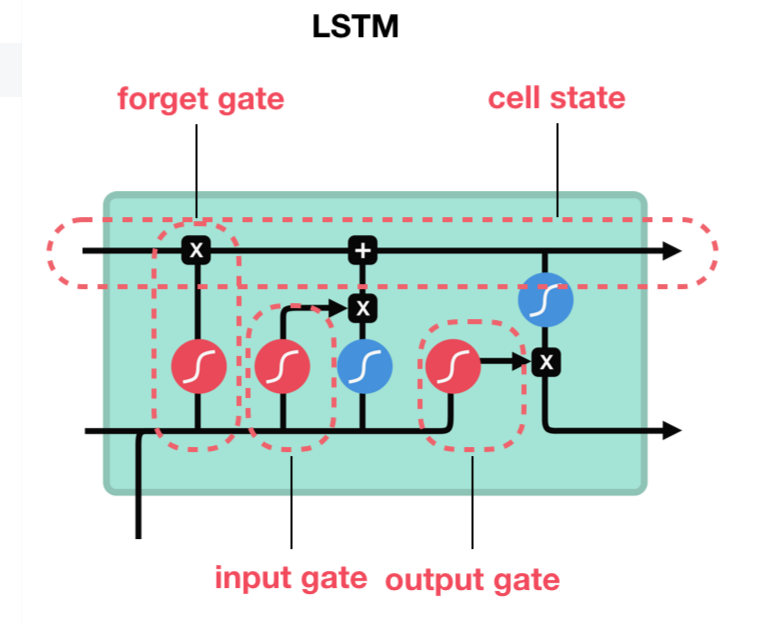
\includegraphics[width=0.5\linewidth]{lstm_gates.png}
    \caption{Przepływ danych w jedynczym neuronie LSTM}
\end{figure}


\subsubsection{Funkcje aktywacji}

Neuron LSTM wykorzystuje dwie funkcje aktywacji:

\begin{itemize}
    \item Tahn (funkcja aktywacji typu tangens hiperboliczny) - pozwala ona na normalizowanie wektora tak by wartości zawierały się w ramach przedziału [-1,1]
    \item Sigmoid (funkcja aktywacji sigmoidalna) - przekształca wartości wektora do wartości z przedziału [0,1]. Istotna z punktu widzenia określania, które elementy wektora powinny zostać zapamiętane (wartość bliżej 1), a które zapomniane (wartość bliżej 0)
\end{itemize}


\subsubsection{Elementy neuronu}

W skład neuronu LSTM wchodzą następujące elementy:
\begin{itemize}
    \item Forget gate
    \item Input gate
    \item Cell state
    \item Output gate
\end{itemize}


\paragraph{Forget gate}  \hfill
%  \break

Zadaniem tej bramy jest decydowanie jaka informacja powinna zostać zachowana przez neuron, a jaka usunięta. Informacje z poprzedniego stanu ukrytego ($h_{t-1}$) i informacje z bieżącego wejścia($x_t$) są przekazywane do sigmoidalnej funkcji aktywacji. Powstała macierz jest oznaczona jako $f_t$. Dla każdej pozycji w macierzy zwracane są wartości z zakresu [0,1]. Im bliżej wartości zero, tym wpływ danej pozycji zanika, im bliżej wartości jeden tym wpływ danej pozycji rośnie.


\paragraph{Input gate}  \hfill

Służy do aktualizacji wewnętrznego stanu neuronu (‘cell state’). Informacje z poprzedniego stanu ukrytego ($h_{t-1}$) i informacje z bieżącego wejścia($x_t$) są przekazywane do sigmoidalnej funkcji aktywacji. Tak jak w przypadku 'forget gate’ uzyskiwana jest macierz o wartościach z zakresu [0,1], która tym razem określa jak bardzo informacja, powstała z połącznia $h_{t-1}$ oraz $x_t$, jest ważna z punktu widzenia zadania klasyfikacji. Wyjście z tej operacji oznaczone jest jako $i_t$.

W ramach tej bramy dokonuje się normalizacja informacji zawartych w ramach połączenia $h_{t-1}$ oraz $x_t$, poprzez wykorzystanie tangensa hiperbolicznego. Wyjście z tej operacji oznaczone jest jako $c_t$.

Kolejnym krokiem jest agregacja informacji z $i_t$ oraz $c_t$ poprzez wykonanie operacji mnożenia macierzy.

\paragraph{Cell state}  \hfill

Ten element neuronu odpowiada za jego stan wewnętrzny i jest przekazywany między kolejnymi komórkami w warstwie. Stan uzyskany z poprzedniej komórki oznaczony jest jako $c_{t-1}$, a z bieżącej jako $c_t$. W celu uzyskania bieżącego stanu komórki wykorzystywane są informacje zgromadzone w ramach poprzednich bram. W pierwszej kolejności dokonywane jest mnożenie macierzowe $c_{t-1}$ oraz $f_t$, które pozwala na usunięcie elementów macierzy nieistotnych z punktu widzenia sieci. Następnie dokonywana jest operacja dodawania uzyskanej macierzy z macierzą uzyskaną w ramach ‘input gate’. Powoduje to dodanie do stanu neuronu nowych informacji istotnych dla sieci. Stan po tej operacji jest określany zmienną $c_t$.


\paragraph{Output gate}  \hfill

Zadaniem tej bramy jest określenie jak powinien wyglądać stan ukryty przekazywany do kolejnego neuronu. Stan ten zawiera informacje na temat poprzednich wejść istotnych z dla zagadnienia klasyfikacji. W ramach tej bramy dokonywane są trzy operacje. Pierwszą z nich jest podanie zagregowanych informacji z poprzedniego stanu ukrytego ($h_{t-1}$) i informacje z bieżącego wejścia($x_t$) na sigmoidalną funkcję aktywacji. W ramach drugiej operacji wewnętrzy stan neuronu (‘cell state’) jest normalizowany przy wykorzystaniu tangesna hiperbolicznego. Trzecią operacją jest mnożenie macierzowe wyników dwóch poprzednich operacji, w efekcie uzyskiwany jest stan ukryty neuronu, oznaczony jako $h_t$, przekazywany do następnego neuronu.

\subsection{Bi-LSTM}

%https://medium.com/@raghavaggarwal0089/bi-lstm-bc3d68da8bd0 

Warstwa składa się z dwóch tak samo zbudowanych warstw LSTM. Jedna z warstw przetwarza ciąg danych wejściowych od początku do końca, a druga od końca do początku. Pozwala to na naukę zależności między elementami w dwóch kierunkach, co przekłada się na większą liczbę informacji na temat sekwencji, co pozwala na szybsze i dokładniejsze trenowanie modelu.





